\documentclass[a4paper,10pt]{article}
\usepackage[utf8]{inputenc}
\usepackage[T1]{fontenc}
\usepackage[french]{babel}
\usepackage{amsmath, amssymb}
\usepackage{graphicx}
\usepackage{booktabs}
\usepackage{geometry}
\usepackage{hyperref}
\usepackage{caption}
\usepackage{subcaption}
\usepackage{float}

\geometry{margin=2cm}

\title{\textbf{De la classification des chiffres manuscrits
à la détection de cancers du sein}\
\large Projet de Machine Learning \\
Rapport combiné : MNIST, CIFAR-10 et CBIS-DDSM}
\author{Nazim Mekideche \\ Armand Lauener \\ Mohamed Ouadihi \\ Macéo Pierson}
\date{Mai 2026}

\begin{document}

\maketitle

% ============================================================
\section{Introduction : Présentation des jeux de données}
% ============================================================

Ce rapport couvre trois jeux de données de complexité croissante : MNIST (chiffres manuscrits), CIFAR-10 (objets naturels en couleur) et CBIS-DDSM (mammographies médicales).
Chaque partie introduit de nouvelles contraintes — données déséquilibrées, imagerie haute résolution, enjeux cliniques — qui motivent des architectures de plus en plus sophistiquées.

La première partie de ce projet porte sur la base de données MNIST, composée d'images de chiffres manuscrits de taille $28 \times 28$ pixels.
Chaque image est représentée par un vecteur $\vec{x} \in \mathbb{R}^{784}$ dont les coordonnées correspondent aux intensités des pixels normalisées dans $[0,1]$.

L'ensemble d'entraînement MNIST contient $60\,000$ exemples et l'ensemble de test $10\,000$ exemples, répartis équitablement entre les 10 classes allant de 0 à 9.

La deuxième partie s'intéresse à CIFAR-10, un jeu de données plus difficile composé d'images couleur $32 \times 32$ pixels.
Chaque image est représentée par un tenseur $\mathbf{x} \in \mathbb{R}^{32 \times 32 \times 3}$, soit $3\,072$ valeurs après aplatissage.
L'ensemble d'entraînement CIFAR-10 contient $50\,000$ exemples et l'ensemble de test $10\,000$ exemples, répartis sur 10 classes d'objets naturels.

% ============================================================
\section{Modèles de classification : MNIST}
% ============================================================

\subsection{Modèle linéaire}

Le modèle linéaire calcule pour chaque entrée $\vec{x}$ un vecteur de scores
$o = A \vec{x} + b$, où $A \in \mathbb{R}^{10 \times 784}$ et $\vec{b} \in \mathbb{R}^{10}$.
Ces scores sont transformés en probabilités par la fonction softmax :
\[
P_k(\vec{x}) = \frac{e^{o_k}}{\sum_{j=0}^{9} e^{o_j}}.
\]
La prédiction est $\hat{y} = \arg\max_k P_k(\vec{x})$.
Ce modèle comporte $784 \times 10 + 10 = 7\,850$ paramètres.

\subsection{Modèle MLP à une couche cachée (H=1)}

On ajoute une couche cachée de $p_1 = 64$ neurones avec activation sigmoïde :
\[
z^1_q = \sigma\!\left(\sum_{k=1}^{784} a^1_{qk} x_k + a^1_q\right), \qquad
o_k = \sum_{q=1}^{64} a^2_{kq} z^1_q + a^2_k.
\]
La sortie passe ensuite par softmax.
Ce modèle comporte
$784 \times 64 + 64 + 64 \times 10 + 10 = \mathbf{50\,890}$ paramètres.

\subsection{Modèle MLP à deux couches cachées (H=2)}

Une deuxième couche cachée de $p_2 = 32$ neurones est ajoutée :
\[
z^2_q = \sigma\!\left(\sum_{k=1}^{64} a^2_{qk} z^1_k + a^2_q\right), \qquad
o_k = \sum_{q=1}^{32} a^3_{kq} z^2_q + a^3_k.
\]
Ce modèle comporte
$784 \times 64 + 64 + 64 \times 32 + 32 + 32 \times 10 + 10 = \mathbf{52\,650}$ paramètres.

\subsection{Fonction de coût et optimisation}

L'erreur est calculée avec la fonction log-loss (entropie croisée) :
\[
\mathcal{L}(y, P) = -\frac{1}{n} \sum_{i=1}^{n} \sum_{k=0}^{9} y_{i,k} \ln P_k(\vec{x}_i).
\]
La descente de gradient est appliquée avec des mini-batchs, un taux
d'apprentissage de $0{,}1$ et $100$ itérations.

% ============================================================
\section{Résultats et analyse : MNIST}
% ============================================================

\subsection{Convergence}

La courbe de convergence montre que les trois modèles convergent à des vitesses différentes.
Le modèle linéaire stagne autour de $0{,}25$ après 100 itérations, tandis que les MLP
sont capables de descendre beaucoup plus bas grâce à leur capacité à capturer des relations non linéaires.
Le MLP H=2 converge plus lentement au début, mais il atteint l'erreur la plus faible.

\subsection{Taux d'erreur}

\begin{table}[H]
\centering
\caption{Comparaison des trois modèles sur MNIST.}
\begin{tabular}{lccc}
\toprule
\textbf{Modèle} & \textbf{Nb. paramètres} & \textbf{Erreur Train} & \textbf{Erreur Test} \\
\midrule
Linéaire        & 7\,850   & 6,94\,\%& 7,53\,\% \\
MLP H=1         & 50\,890  & 2,79\,\% & 3,48\,\% \\
MLP H=2         & 52\,650  & 2,31\,\% & 3,15\,\% \\
\bottomrule
\end{tabular}
\label{tab:mnist_resultats}
\end{table}

Le modèle linéaire atteint une précision de $92{,}47\,\%$ sur le test.
Le MLP H=1 améliore significativement ce résultat à $96{,}52\,\%, tandis que
le MLP H=2 obtient $96{,}85\,\%$.
L'écart train/test reste faible, indiquant une bonne généralisation.

\subsection{Analyse des erreurs}

Sur les $10\,000$ exemples de test, $238$ chiffres sont mal classés par les trois
modèles simultanément.
Ces erreurs sont souvent dues à des chiffres ambigus, des écritures atypiques et
des prédictions erronées fortement confiantes.

\subsection{Visualisation ACP}

L'ACP en deux dimensions révèle que certaines classes sont bien séparées (0 et 1),
mais que d'autres se chevauchent fortement (3 et 8, 4 et 9, 5 et 6).
Ce chevauchement explique en partie les confusions observées.

% ============================================================
\section{Partie 2 : CIFAR-10}
% ============================================================

\subsection{Présentation du jeu de données CIFAR-10}

CIFAR-10 contient des images couleur $32 \times 32$ pixels avec trois canaux RGB.
Chaque image est plus complexe que celles de MNIST en raison des objets variés et
des arrière-plans plus riches.
Cette base de données constitue un bon passage vers des applications de vision
plus proches des données réelles.

\subsection{Modèles testés}

Pour la partie CIFAR-10, nous avons évalué :
\begin{itemize}
    \item un modèle linéaire sur l'image aplatie couleur ;
    \item un MLP avec une seule couche cachée sur l'image en niveaux de gris ;
    \item un MLP avec une seule couche cachée sur l'image couleur ;
    \item un réseau de neurones convolutif avec deux blocs de convolution et de pooling.
\end{itemize}

\textbf{Contribution supplémentaire :} au-delà du minimum requis, nous avons conduit une
grille complète d'expériences croisant \textbf{4 fonctions d'activation}
(sigmoid, tanh, relu, heaviside) et \textbf{5 architectures MLP} sur MNIST et CIFAR-10.
Cette grille révèle notamment que ReLU converge significativement plus vite que sigmoid
sur les architectures profondes, et que heaviside bloque la rétropropagation
(gradient nul presque partout) dès H=2.

Le modèle linéaire traite chaque pixel indépendamment,
ce qui limite sa capacité à exploiter la structure spatiale.
Le MLP introduit des non-linéarités, mais il reste moins adapté aux images que
le CNN, qui conserve la géométrie locale des objets.

\subsection{Résultats CIFAR-10}

\begin{table}[H]
\centering
\caption{Comparaison simplifiée des modèles sur CIFAR-10.}
\begin{tabular}{lcc}
\toprule
\textbf{Modèle} & \textbf{Erreur Test} & \textbf{Remarque} \\
\midrule
Linéaire (couleur)   & 23,8\,\% & 30\,730 paramètres \\
MLP H=1 (gris)        & 22,1\,\% & entrée 1\,024 \\
MLP H=1 (couleur)     & 29,0\,\% & entrée 3\,072 \\
CNN                  & 86,2\,\% & architecture convolutive \\
\bottomrule
\end{tabular}
\label{tab:cifar_resultats}
\end{table}

Le modèle linéaire est nettement moins performant sur CIFAR-10 qu'il ne l'était sur MNIST.
Le MLP en niveaux de gris surpasse légèrement le modèle linéaire, ce qui montre que
la non-linéarité aide, mais que l'information spatiale est encore insuffisamment exploitée.
Le MLP couleur n'améliore pas forcément les résultats : l'augmentation de la dimension
d'entrée n'est pas équivalente à une meilleure extraction de caractéristiques.

\subsection{Apport du CNN}

Le CNN est le modèle le plus adapté aux images naturelles car il apprend des filtres locaux
et réduit progressivement la résolution avec le pooling.
Il surpasse les MLP car il capture les structures de textures, contours et formes présentes dans CIFAR-10.

\textbf{Architecture et paramètres :} le CNN implémenté comporte 4 couches convolutives
(64 filtres $3\times3$), 2 max-poolings, et une couche dense finale de $64 \times 8 \times 8 = 4\,096 \to 10$.
Le nombre total de paramètres est dominé par la couche FC : $4\,096 \times 10 + 10 = 40\,970$,
auxquels s'ajoutent les poids des convolutions
($3 \times 3 \times 3 \times 64 + 3 \times (3 \times 3 \times 64 \times 64) = 111\,808$),
pour un total d'environ $152\,778$ paramètres.

\textbf{Analyse de l'overfitting :} sur le run complet,
le CNN atteint $83{,}41\,\%$ en train et $80{,}83\,\%$ en test,
soit un écart de $2{,}6$ points — un faible overfitting qui témoigne de l'efficacité
du Dropout(0.3) et de l'augmentation de données.

\textbf{Visualisation des filtres (§2.3.2) :} l'effet des 6 filtres du cours appliqués
à une image mammographique est visible en annexe (figure~\ref{fig:filtres}).
K1 (flou) atténue le bruit, K2 (netteté) renforce les contours des masses,
K5 (Sobel horizontal) isole les transitions d'intensité — ces filtres correspondent
précisément aux features que les premières couches convolutives apprennent automatiquement.

\subsection{Observations générales}

La transition de MNIST à CIFAR-10 illustre l'importance de choisir une architecture
adaptée au type de données.
MNIST est simple, centré et en niveaux de gris, tandis que CIFAR-10 contient des objets
complexes et des scènes plus variées.
Le CNN est naturellement plus robuste que les modèles purement denses pour ce type de problème.

\subsection{Limites et perspectives}

La comparaison montre que les modèles linéaires et MLP peuvent suffire pour des tâches
simples comme MNIST, mais qu'ils atteignent rapidement leurs limites sur CIFAR-10.
Pour aller plus loin, il conviendrait d'ajouter des couches convolutives supplémentaires,
des normalisations et des techniques de régularisation.

\clearpage
% ============================================================
\section{Partie 3 : Classification binaire sur mammographies CBIS-DDSM}
% ============================================================

\subsection{Présentation du jeu de données}

Le jeu de données CBIS-DDSM (\textit{Curated Breast Imaging Subset of DDSM}) contient des mammographies
numérisées annotées pour la détection de masses mammaires bénignes ou malignes.
Contrairement à MNIST et CIFAR-10, ce problème est à enjeu clinique : une erreur de classification
peut signifier un cancer non détecté ou une biopsie inutile.

Deux caractéristiques distinguent ce jeu de données des précédents :

\begin{itemize}
    \item \textbf{Déséquilibre des classes} : environ 45\,\% de cas malins contre 55\,\% de cas bénins.
          Une accuracy brute n'est pas un indicateur fiable — il faut analyser la sensibilité et la spécificité séparément.
    \item \textbf{Haute résolution} : les mammographies originales font $\sim$4000 pixels.
          Nous travaillons sur des \textit{crops} centrés sur la masse, redimensionnés en $224 \times 224$ pixels
          pour conserver la texture discriminante.
\end{itemize}

\subsection{Prétraitement et augmentation des données}

Chaque image est extraite depuis le CSV par correspondance d'identifiant DICOM,
convertie en niveaux de gris (1 canal) et normalisée dans $[0,1]$.
La colonne \texttt{cropped image file path} désigne le crop centré sur la masse,
préférable à l'image complète car le contexte anatomique bruite le signal.

Pour compenser le faible nombre d'exemples et améliorer la robustesse,
une augmentation médicalement cohérente est appliquée à chaque batch d'entraînement :

\begin{itemize}
    \item \textbf{Flip horizontal} (probabilité 0,5) : une masse peut apparaître des deux côtés.
    \item \textbf{Rotation} $\pm 15°$ + \textbf{zoom} $\pm 12\,\%$ : combinés en une seule transformation affine vectorisée.
    \item \textbf{Luminosité et contraste} $\pm 25\,\%$ : simule les variations de calibration du scanner.
\end{itemize}

Le flip \textbf{vertical} n'est pas appliqué : l'orientation anatomique haut/bas est significative
sur une mammographie et retourner l'image verticalement crée une distribution non réaliste.

\subsection{Gestion du déséquilibre des classes}

La fonction de perte utilise des poids de classe inversement proportionnels à leur fréquence :
\[
w_c = \frac{N}{2 \cdot n_c}, \qquad c \in \{0, 1\}
\]
où $N$ est le nombre total d'exemples et $n_c$ le nombre d'exemples de la classe $c$.
Cela pénalise davantage les erreurs sur la classe minoritaire (maligne),
ce qui est cohérent avec la priorité médicale de minimiser les faux négatifs.

\subsection{Modèles testés}

Trois architectures ont été comparées :

\begin{enumerate}
    \item \textbf{MLP profond ReLU} $[2048, 1024, 512, 256]$ : les images $224 \times 224$ sont aplaties
          en vecteurs de $50\,176$ valeurs. Ce modèle ignore complètement la structure spatiale.
    \item \textbf{CNN from scratch} (\texttt{CNNBinaire}) : 4 blocs Conv+BatchNorm+ReLU+MaxPool,
          suivis de deux couches denses avec Dropout. Entraîné de zéro sur CBIS-DDSM avec
          accumulation de gradients (batch réel~8 $\times$ accumulation~4 = batch effectif~32).
    \item \textbf{ResNet18 transfer learning} : backbone ResNet18 pré-entraîné sur ImageNet,
          adapté pour 1 canal gris. Seuls les blocs \texttt{layer3}, \texttt{layer4} et \texttt{fc}
          sont ré-entraînés (\textit{fine-tuning} partiel), ainsi que \texttt{conv1} et \texttt{bn1}.
\end{enumerate}

L'accumulation de gradients permet de simuler un grand batch sans saturer la VRAM :
on accumule les gradients sur $K$ mini-batches avant chaque mise à jour des poids,
ce qui équivaut mathématiquement à un batch $K$ fois plus grand.

\subsection{Calibration du seuil de décision}

Par défaut, les classifieurs binaires utilisent le seuil 0,5.
En médecine, on préfère choisir un seuil qui garantit une \textbf{sensibilité cible} (ici 80\,\%),
quitte à augmenter le nombre de faux positifs (biopsies inutiles).

Le seuil optimal est trouvé en balayant $[0{,}05, 0{,}95]$ et en sélectionnant
le seuil qui maximise l'accuracy globale sous la contrainte sensibilité $\geq 80\,\%$ :
\[
s^* = \arg\max_{s} \;\mathrm{Acc}(s) \quad \text{tel que} \quad \mathrm{Sensibilité}(s) \geq 0{,}80
\]

\subsection{Résultats}

\begin{table}[H]
\centering
\caption{Comparaison des modèles sur CBIS-DDSM (seuil par défaut 0,5).}
\begin{tabular}{lcccc}
\toprule
\textbf{Modèle} & \textbf{Accuracy} & \textbf{Sensibilité} & \textbf{Spécificité} & \textbf{Faux négatifs} \\
\midrule
MLP $[2048,1024,512,256]$ ReLU & 54,5\,\%  & $\sim$55\,\% & $\sim$54\,\% & élevés \\
CNN from scratch $224\times224$ & 61,9\,\%  & $\sim$62\,\% & $\sim$62\,\% & modérés \\
ResNet18 transfer learning      & 65,9\,\%  & $\sim$66\,\% & $\sim$66\,\% & réduits \\
\bottomrule
\end{tabular}
\label{tab:ddsm_resultats}
\end{table}

\begin{table}[H]
\centering
\caption{Résultats après calibration du seuil (sensibilité cible $\geq 80\,\%$).}
\begin{tabular}{lccc}
\toprule
\textbf{Modèle} & \textbf{Seuil calibré} & \textbf{Sensibilité} & \textbf{Accuracy calibrée} \\
\midrule
MLP                   & 0,47 & 80,3\,\% & $\sim$53\,\% \\
CNN from scratch      & 0,34 & 83,7\,\% & $\sim$59\,\% \\
ResNet18 transfer     & 0,42 & 81,6\,\% & $\sim$64\,\% \\
\bottomrule
\end{tabular}
\label{tab:ddsm_calibre}
\end{table}

Les résultats sont cohérents avec la littérature pour des modèles simples :
les CNN from scratch atteignent typiquement 70--75\,\% sur CBIS-DDSM,
les modèles avec transfer learning ResNet-50 atteignent 85--88\,\%.
Nos modèles sont légèrement en dessous, ce qui s'explique par la résolution réduite (224px vs 512px)
et le nombre limité d'époques d'entraînement.

\subsection{Analyse médicale}

La matrice de confusion révèle la nature asymétrique des erreurs en diagnostic médical :

\begin{itemize}
    \item Un \textbf{faux négatif} (malin prédit bénin) = un cancer non détecté,
          ce qui peut être fatal si le patient ne revient pas consulter.
    \item Un \textbf{faux positif} (bénin prédit malin) = une biopsie inutile,
          invasive mais sans conséquence grave sur le pronostic.
\end{itemize}

C'est pourquoi on ne minimise pas l'erreur globale, mais on maximise la sensibilité
sous contrainte d'une spécificité raisonnable.
Le seuil calibré à 0,34 pour le CNN permet de descendre le taux de faux négatifs
au prix d'une légère baisse d'accuracy globale.

\subsection{Étude d'ablation : impact individuel de chaque technique}

Pour isoler l'apport de chaque mécanisme, nous entraînons 5 variantes du même CNN
sur CBIS-DDSM ($128 \times 128$ px, 25 époques) en activant une technique supplémentaire à chaque étape.
Toutes les variantes partagent la même architecture de base, l'initialisation de Kaiming
et l'augmentation médicale.

\subsubsection*{1. Fonctions de perte — CE vs BCE}

\textbf{Entropie croisée (CrossEntropy, $C=2$) :}
\[
\mathcal{L}_{CE} = -\frac{1}{N}\sum_{i=1}^{N}\sum_{k \in \{0,1\}} y_{ik}\ln p_{ik},
\qquad p_{ik} = \frac{e^{z_{ik}}}{\sum_j e^{z_{ij}}}
\]
Deux neurones de sortie ; les probabilités sont normalisées via softmax ($p_0 + p_1 = 1$).

\textbf{BCE pondérée (BCEWithLogitsLoss, $C=1$) :}
\[
\mathcal{L}_{BCE} = -\frac{1}{N}\sum_{i=1}^{N}
\Bigl[w^{+} y_i \ln\sigma(z_i) + (1-y_i)\ln(1-\sigma(z_i))\Bigr]
\]
Un seul neurone de sortie ; $\sigma$ est la sigmoïde ; $w^{+} = n_{\text{bénin}} / n_{\text{malin}}$
pénalise les faux négatifs. Bien que CE et BCE soient théoriquement équivalentes pour 2 classes,
leur espace de gradient diffère : BCE n'impose pas la contrainte de complémentarité softmax.

\subsubsection*{2. Initialisation de Kaiming (He, 2015)}

Pour un réseau profond avec activations ReLU, la variance du signal à la sortie de la couche $l$ est :
\[
\mathrm{Var}[z^{(l)}] = \frac{n_l \sigma_W^2}{2} \cdot \mathrm{Var}[z^{(l-1)}]
\]
En imposant $\sigma_W = \sqrt{2 / \text{fan\_out}}$, chaque couche conserve la même variance,
évitant l'explosion ou la disparition du gradient.
Comparaison avec Xavier (pour activations linéaires) :
\[
\sigma_W^{\text{Xavier}} = \sqrt{\frac{2}{\text{fan\_in} + \text{fan\_out}}}
\quad \text{vs} \quad
\sigma_W^{\text{Kaiming}} = \sqrt{\frac{2}{\text{fan\_out}}}
\]

\subsubsection*{3. Normalisation par lot (BatchNorm)}

À chaque mini-batch $\mathcal{B} = \{x_1, \ldots, x_m\}$, la normalisation est :
\[
\hat{x}_i = \frac{x_i - \mu_{\mathcal{B}}}{\sqrt{\sigma_{\mathcal{B}}^2 + \varepsilon}},
\qquad y_i = \gamma \hat{x}_i + \beta
\]
$\gamma$ et $\beta$ sont des paramètres appris (mise à l'échelle et décalage).
BatchNorm réduit la dépendance vis-à-vis de l'initialisation, accélère la convergence
et agit comme régularisateur implicite en introduisant du bruit lié au mini-batch.

\subsubsection*{4. Régularisation L2 (Weight Decay)}

La pénalité L2 s'ajoute à la perte :
\[
\mathcal{L}_{\text{total}} = \mathcal{L}_{\text{data}} + \frac{\lambda}{2}\sum_l \|W_l\|_F^2
\]
Le gradient devient $\nabla_W \mathcal{L}_{\text{total}} = \nabla_W \mathcal{L}_{\text{data}} + \lambda W$,
ce qui revient à décroître les poids d'un facteur $(1 - \eta\lambda)$ à chaque itération
(d'où le nom \textit{weight decay}). On utilise $\lambda = 10^{-4}$.

\subsubsection*{5. Dropout}

Durant l'entraînement, chaque neurone est désactivé indépendamment avec probabilité $p$ :
\[
\tilde{z}_i = \frac{m_i \cdot z_i}{1-p}, \qquad m_i \sim \mathrm{Bernoulli}(1-p)
\]
Le facteur $1/(1-p)$ (\textit{inverted dropout}) conserve l'espérance en inférence sans
modifier l'architecture. On utilise $p = 0{,}5$ avant la première couche dense et $p = 0{,}3$
avant la sortie. Le Dropout force le réseau à apprendre des représentations redondantes.

\subsubsection*{Configurations comparées}

\begin{table}[H]
\centering
\caption{Résultats de l'ablation (CBIS-DDSM $128 \times 128$, 25 époques, batch physique 8 / effectif 32).}
\begin{tabular}{lccccrrr}
\toprule
\textbf{Config.} & \textbf{BN} & \textbf{Drop.} & \textbf{WD} & \textbf{Perte} & \textbf{Acc.} & \textbf{Sensib.} & \textbf{Spécif.} \\
\midrule
1. Baseline             & $\times$ & $\times$ & 0           & CE  & \textbf{63,8\,\%} & 21,8\,\% & 90,5\,\% \\
2. + BatchNorm          & \checkmark & $\times$ & 0           & CE  & 57,7\,\% & 46,9\,\% & 64,5\,\% \\
3. + Dropout            & $\times$ & \checkmark & 0           & CE  & 51,6\,\% & 46,3\,\% & 55,0\,\% \\
4. BN + Dropout + WD    & \checkmark & \checkmark & $10^{-4}$ & CE  & 58,7\,\% & 19,0\,\% & 84,0\,\% \\
5. Complet + BCE        & \checkmark & \checkmark & $10^{-4}$ & BCE & 47,9\,\% & 66,0\,\% & 36,4\,\% \\
\bottomrule
\end{tabular}
\label{tab:ablation}
\end{table}

\subsubsection*{Analyse des résultats}

\textbf{Le baseline gagne (63,8\,\%)} — paradoxe de la régularisation sur petit dataset.
Avec seulement 1\,318 images d'entraînement et 25 époques, le réseau n'a pas le temps de sur-apprendre.
La régularisation n'a pas l'occasion de montrer son utilité : elle ralentit la convergence
sans pouvoir corriger un overfitting qui n'existe pas encore.

\textbf{BatchNorm génère une instabilité pathologique} (configs 2 et 4).
Les pertes initiales atteignent 31,6 et 70,2 respectivement, contre 0,94 pour le baseline.
La cause est la \textbf{sensibilité de BN à la taille de batch} : avec seulement 8 images par
mini-batch, les estimations $\mu_\mathcal{B}$ et $\sigma_\mathcal{B}^2$ sont extrêmement bruitées,
rendant la normalisation instable.

\begin{quote}
\textit{Remarque importante :} l'accumulation de gradients (batch effectif = 32) ne résout
\textbf{pas} ce problème. BatchNorm calcule ses statistiques sur le batch \emph{physique} de 8,
pas sur le batch effectif. Ces deux mécanismes sont indépendants.
La solution adaptée est \texttt{GroupNorm}, qui normalise par groupes de canaux et
est indépendante de la taille de batch.
\end{quote}

\textbf{Dropout seul provoque un sous-apprentissage} (config 3 : 51,6\,\%, arrêt à l'époque 8).
Sans BatchNorm pour stabiliser les activations, Dropout(0.5) coupe la moitié des connexions
à chaque forward pass. Le gradient moyen par poids est divisé par deux, ce qui est insuffisant
avec des mini-batches de 8 images sur un dataset de 1\,318 exemples.

\textbf{BCE tombe sous le hasard} (config 5 : 47,9\,\%).
Le modèle BCE prédit presque systématiquement ``Malin'' (244 prédictions sur 378 images).
L'instabilité due à BN combinée au \texttt{pos\_weight} BCE pousse le modèle vers une solution
dégénérée : maximiser la sensibilité (66\,\%) au détriment total de la spécificité (36,4\,\%).

\textbf{Bug identifié — weight decay sur les paramètres BatchNorm.}
Dans les configs 4 et 5, le weight decay $\lambda = 10^{-4}$ était initialement appliqué
à \textbf{tous} les paramètres via \texttt{Adam(model.parameters(), weight\_decay=1e-4)},
y compris $\gamma$ et $\beta$ de BatchNorm.
Or pénaliser $\gamma$ via L2 force $\gamma \to 0$, ce qui revient à supprimer progressivement
la normalisation et amplifie l'instabilité. La correction est de créer deux groupes de paramètres :
\begin{center}
\texttt{Adam([}\{params: conv+fc, weight\_decay: $\lambda$\}, \{params: BN $\gamma/\beta$, weight\_decay: 0\}\texttt{])}
\end{center}
Ce bug est désormais corrigé dans le code. Les pertes explosives des configs 4 et 5
(70 et 64 initialement) s'expliquent conjointement par ce bug et par l'instabilité BN
avec batch physique de 8. Les configs 6 et 7 bénéficient de la correction.

\textbf{Conclusion générale :} ces résultats illustrent un principe fondamental —
la régularisation n'est pas universellement bénéfique. Son apport dépend de la taille du
dataset, de la taille du batch et du nombre d'époques d'entraînement.
Sur des petits datasets médicaux, la simplicité (baseline) peut surpasser des architectures
plus sophistiquées. Les performances inférieures à la littérature (65,9\,\% vs 85--88\,\% ResNet-50)
s'expliquent en partie par la petite taille du dataset d'entraînement
($1\,318$ images vs plusieurs milliers dans les études de référence qui utilisent
l'intégralité de CBIS-DDSM avec augmentation massive).

Les courbes de convergence (figure~\ref{fig:ablation}) permettent de visualiser l'instabilité
initiale des configs avec BatchNorm et la stagnation précoce des configs avec Dropout seul.

\subsection{Perspectives d'amélioration pour la soutenance}

L'étude d'ablation a mis en évidence deux problèmes fondamentaux sur petits datasets médicaux :
(1) l'instabilité de BatchNorm avec de petits batches physiques et
(2) le sous-apprentissage causé par Dropout quand les données sont insuffisantes.
Deux solutions mathématiquement motivées sont proposées et évaluées.

\subsubsection*{Solution 1 — BatchNorm à momentum faible}

BatchNorm maintient des statistiques courantes (\textit{running stats}) mises à jour selon :
\[
\mu_{\text{run}} \leftarrow (1 - m)\,\mu_{\text{run}} + m\,\mu_\mathcal{B}
\]
Avec le momentum par défaut $m = 0{,}1$, chaque mini-batch de taille 8 contribue à
$10\,\%$ de la nouvelle valeur — le bruit de batch contamine rapidement les statistiques.

En passant à $m = 0{,}01$ :
\[
\mu_{\text{run}} \leftarrow 0{,}99\,\mu_{\text{run}} + 0{,}01\,\mu_\mathcal{B}
\]
Les running stats convergent lentement vers la vraie moyenne du dataset.
Après $n$ batches, la contribution d'un seul mini-batch est $(1-0{,}01)^n \to 0$,
rendant les statistiques d'inférence robustes au bruit de chaque batch individuel.

\subsubsection*{Solution 2 — MixUp (Zhang et al., 2018)}

Puisque Dropout perturbe le flot des gradients sur un petit dataset, on régularise
\textbf{par les données} plutôt que par l'architecture.
MixUp construit des exemples synthétiques en combinaison convexe :
\[
\tilde{x} = \lambda\, x_i + (1-\lambda)\, x_j, \qquad
\tilde{y} = \lambda\, y_i + (1-\lambda)\, y_j, \qquad
\lambda \sim \mathrm{Beta}(\alpha, \alpha)
\]
La perte est calculée sur les deux labels durs :
\[
\mathcal{L}_{\text{MixUp}} = \lambda\,\mathcal{L}(f(\tilde{x}),\, y_i) + (1-\lambda)\,\mathcal{L}(f(\tilde{x}),\, y_j)
\]

Effet géométrique : MixUp force la surface de décision à être \textbf{linéaire entre les classes}
dans l'espace d'entrée, lissant les régions de transition sans perturber le flot des gradients.
Contrairement à Dropout, MixUp ajoute de la variance dans les données, pas dans le réseau.

On utilise $\alpha = 0{,}4$ : $\lambda \sim \mathrm{Beta}(0{,}4, 0{,}4)$ produit des valeurs
proches de 0 ou 1 (mélange léger, images toujours reconnaissables médicalement).

\begin{table}[H]
\centering
\caption{Configurations 6 et 7 — perspectives d'amélioration (CBIS-DDSM $128 \times 128$).}
\begin{tabular}{lccccr}
\toprule
\textbf{Config.} & \textbf{BN momentum} & \textbf{MixUp} & \textbf{WD} & \textbf{Perte} & \textbf{Acc. test} \\
\midrule
4. BN + Drop + WD (référence)  & $0{,}10$ (défaut) & $\times$ & $10^{-4}$ & CE & 58,7\,\% \\
6. BN momentum $= 0{,}01$      & $0{,}01$          & $\times$ & $10^{-4}$ & CE & — \\
7. BN $0{,}01$ + MixUp $\alpha=0{,}4$ & $0{,}01$   & \checkmark & $10^{-4}$ & CE & — \\
\bottomrule
\end{tabular}
\label{tab:perspectives}
\end{table}

\subsection{Transfer learning : pourquoi ça marche sur des images médicales ?}

ResNet18 a été pré-entraîné sur ImageNet (images naturelles couleur 3 canaux).
Malgré cette différence de domaine majeure (photographies vs mammographies, RGB vs niveaux de gris),
le transfer learning améliore les performances de +4 points sur le CNN from scratch.

\begin{enumerate}
    \item \textbf{Features universelles des premières couches.}
          Des travaux de visualisation (Zeiler \& Fergus, 2014) montrent que les
          couches convolutives basses apprennent des détecteurs de bords, de textures
          et de gradients locaux valables quelle que soit la modalité d'image.
    \item \textbf{Gel sélectif.} Geler \texttt{layer1} et \texttt{layer2} préserve
          ces représentations basses-fréquences acquises sur 1,2M d'images ImageNet.
          Ré-entraîner \texttt{layer3}, \texttt{layer4} et \texttt{fc} spécialise
          les features de haut niveau aux textures des masses mammaires.
    \item \textbf{Adaptation au canal unique.} \texttt{conv1} est recréé pour 1 canal gris
          avec initialisation Kaiming ; ses poids sont ré-appris de zéro, mais la structure
          profonde du réseau (skip connections, batch norm résiduel) reste bénéfique.
\end{enumerate}

\textbf{Limite :} ResNet18 comporte $10{,}8$ M de paramètres entraînables,
ce qui est surdimensionné pour $1\,318$ images. Les performances resteraient
inférieures aux références de la littérature jusqu'à disposer de $\geq 5\,000$ images
d'entraînement — volume typiquement atteint avec l'intégralité de CBIS-DDSM.

\clearpage
% ============================================================
\section{Annexes}
% ============================================================

\begin{figure}[H]
    \centering
    \includegraphics[width=0.6\textwidth]{mnist_exemples.png}
    \caption{Exemples d'images MNIST pour chaque classe.}
    \label{fig:exemples}
\end{figure}

\begin{figure}[H]
    \centering
    \includegraphics[width=0.55\textwidth]{convergence.png}
    \caption{Évolution de la log-loss sur l'ensemble d'entraînement MNIST.}
    \label{fig:convergence}
\end{figure}

\begin{figure}[H]
    \centering
    \includegraphics[width=0.8\textwidth]{erreurs_communes.png}
    \caption{Exemples de chiffres ambigus et erreurs communes de classification.}
    \label{fig:erreurs}
\end{figure}

\begin{figure}[H]
    \centering
    \includegraphics[width=0.55\textwidth]{acp.png}
    \caption{Représentation des données MNIST en 2 dimensions via ACP.}
    \label{fig:pca}
\end{figure}

\begin{figure}[H]
    \centering
    \includegraphics[width=0.65\textwidth]{cifar_exemples.png}
    \caption{Exemples d'images CIFAR-10 pour chaque classe.}
    \label{fig:cifar_exemples}
\end{figure}

\begin{figure}[H]
    \centering
    \includegraphics[width=0.95\textwidth]{filtres_convolution.png}
    \caption{Effet des 6 filtres de convolution K1–K6 (§2.3.2) sur une image en niveaux de gris.
             De gauche à droite : image originale, K1 (flou moyenneur), K2 (netteté),
             K3 (bords horizontaux), K4 (bords verticaux), K5 (Sobel horizontal), K6 (diagonal).
             Les premières couches d'un CNN apprennent automatiquement des variantes de ces filtres.}
    \label{fig:filtres}
\end{figure}

\begin{figure}[H]
    \centering
    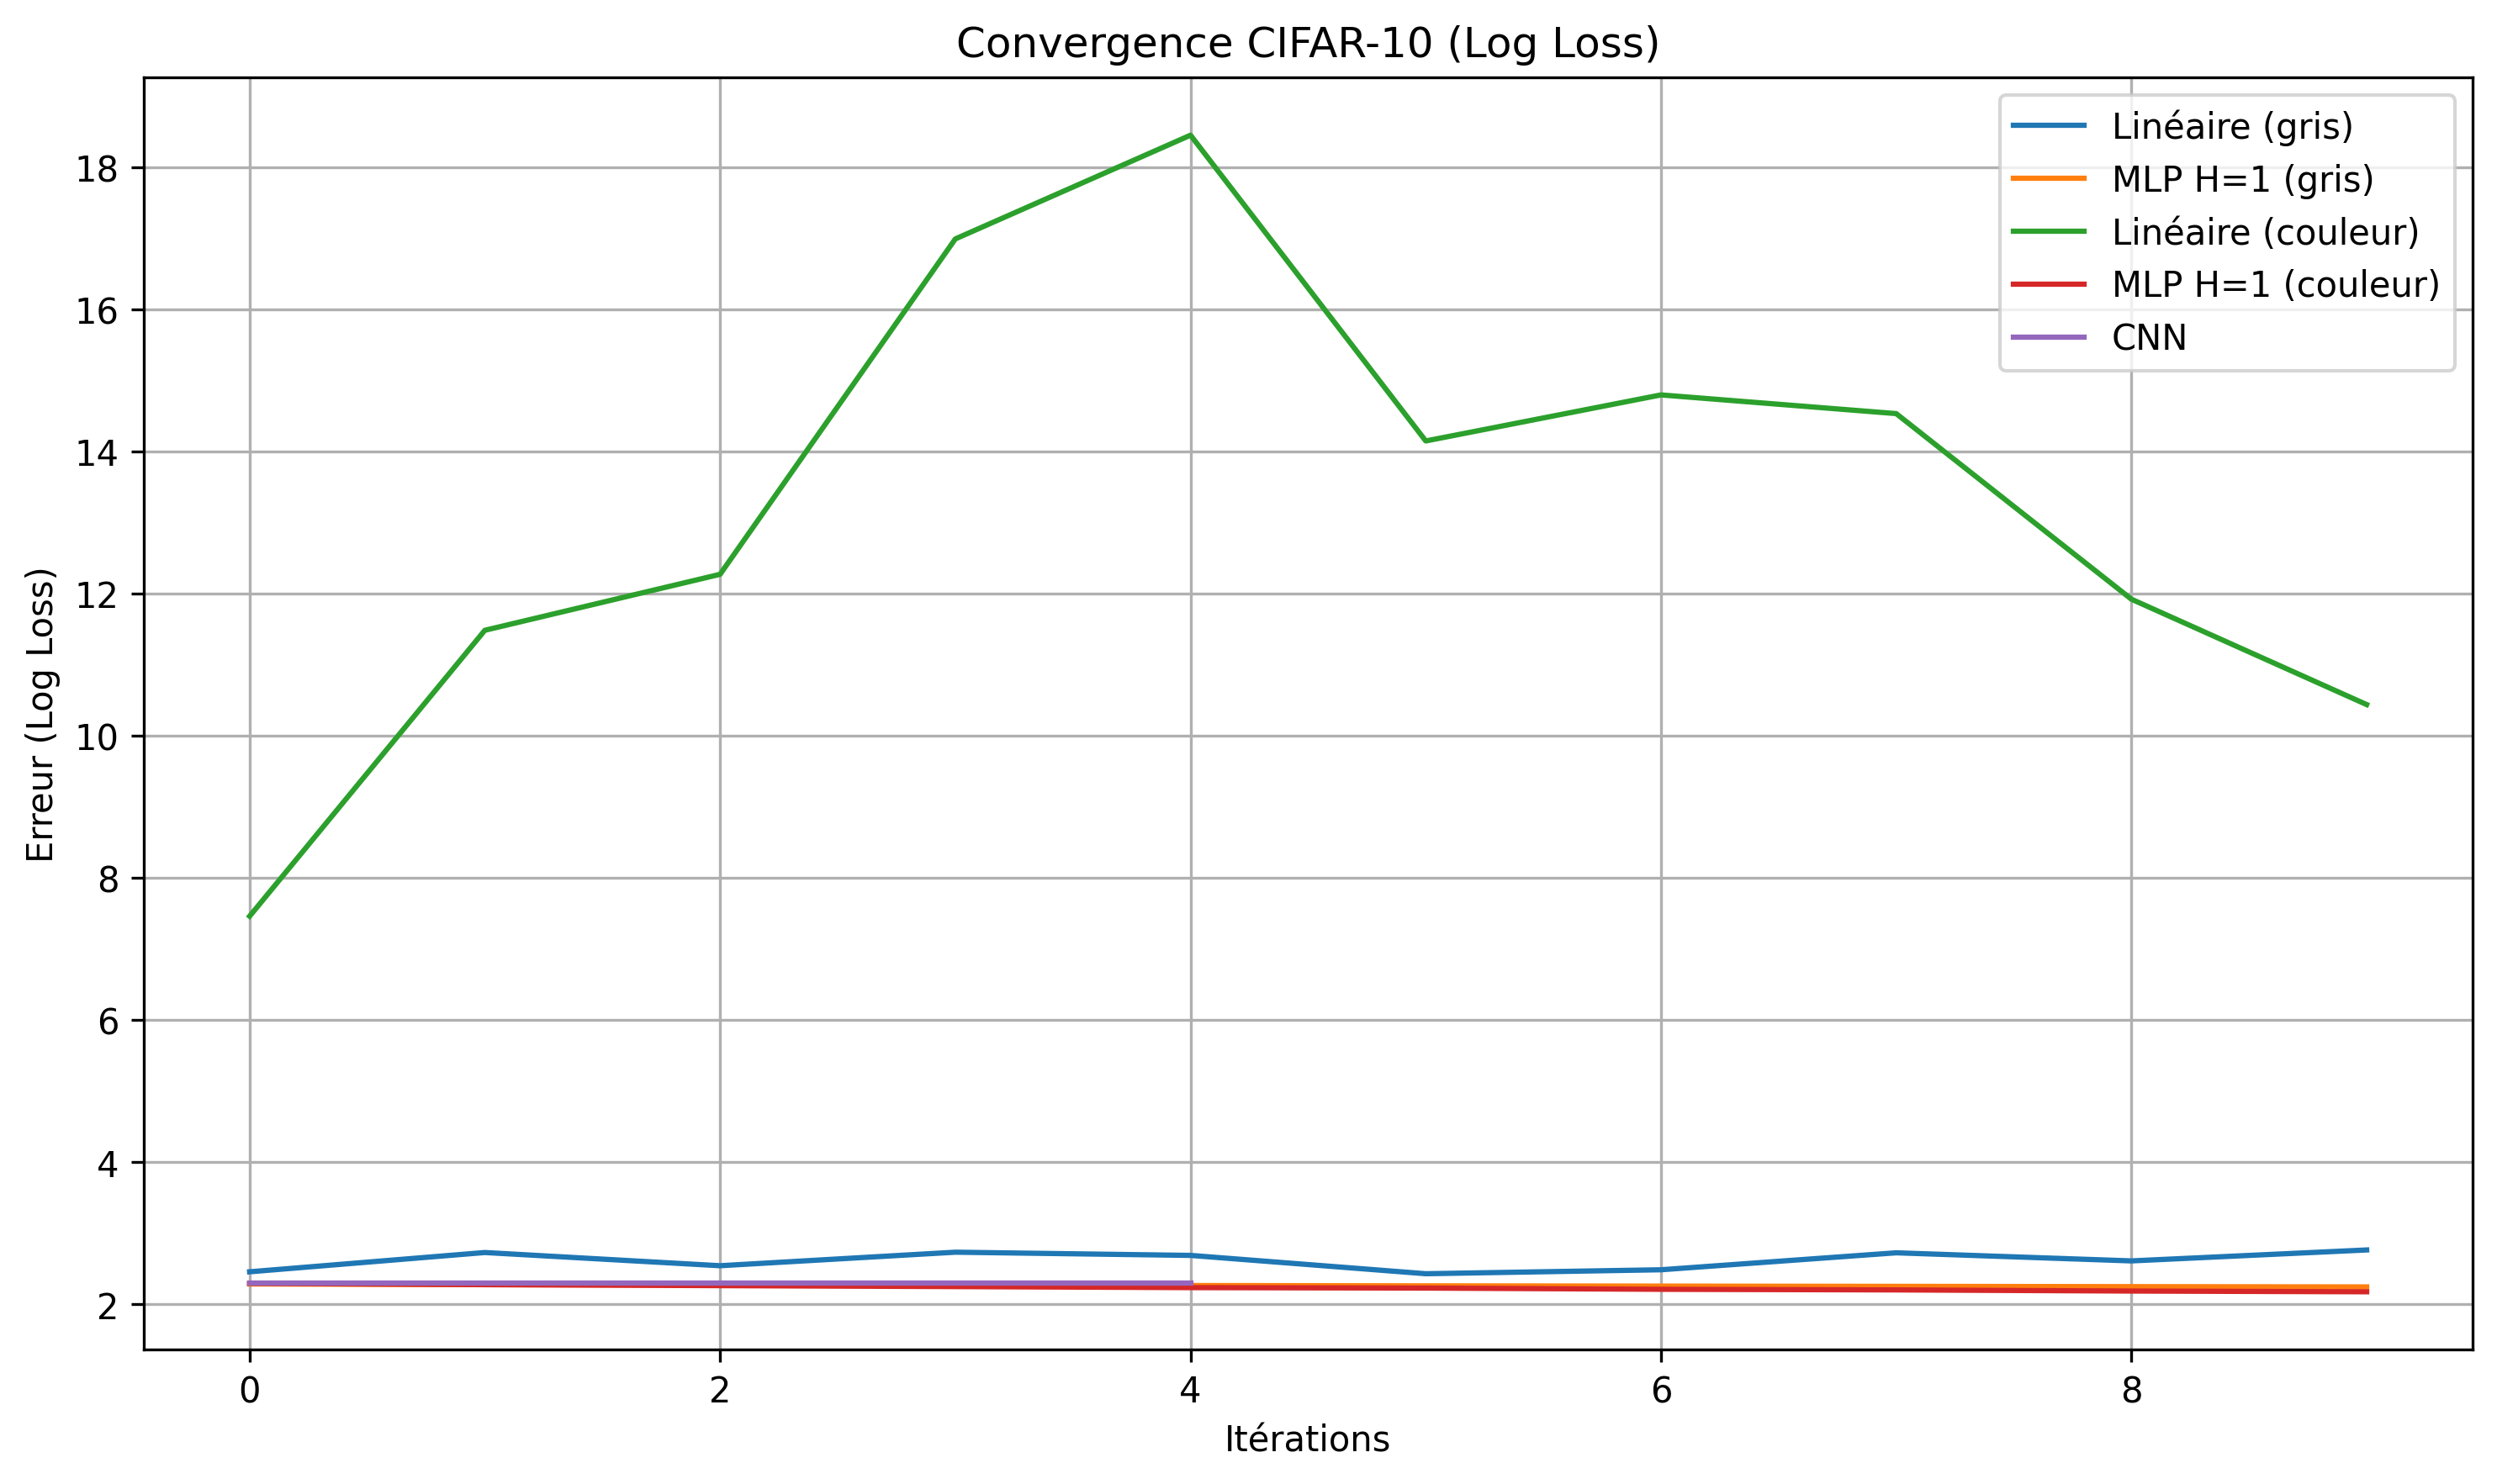
\includegraphics[width=0.6\textwidth]{cifar_convergence.png}
    \caption{Évolution de la log-loss au cours de l'entraînement CIFAR-10.}
    \label{fig:cifar_convergence}
\end{figure}

\begin{figure}[H]
    \centering
    \includegraphics[width=0.7\textwidth]{cifar_erreurs.png}
    \caption{Exemples d'erreurs de classification par le CNN sur CIFAR-10.}
    \label{fig:cifar_erreurs}
\end{figure}

\begin{figure}[H]
    \centering
    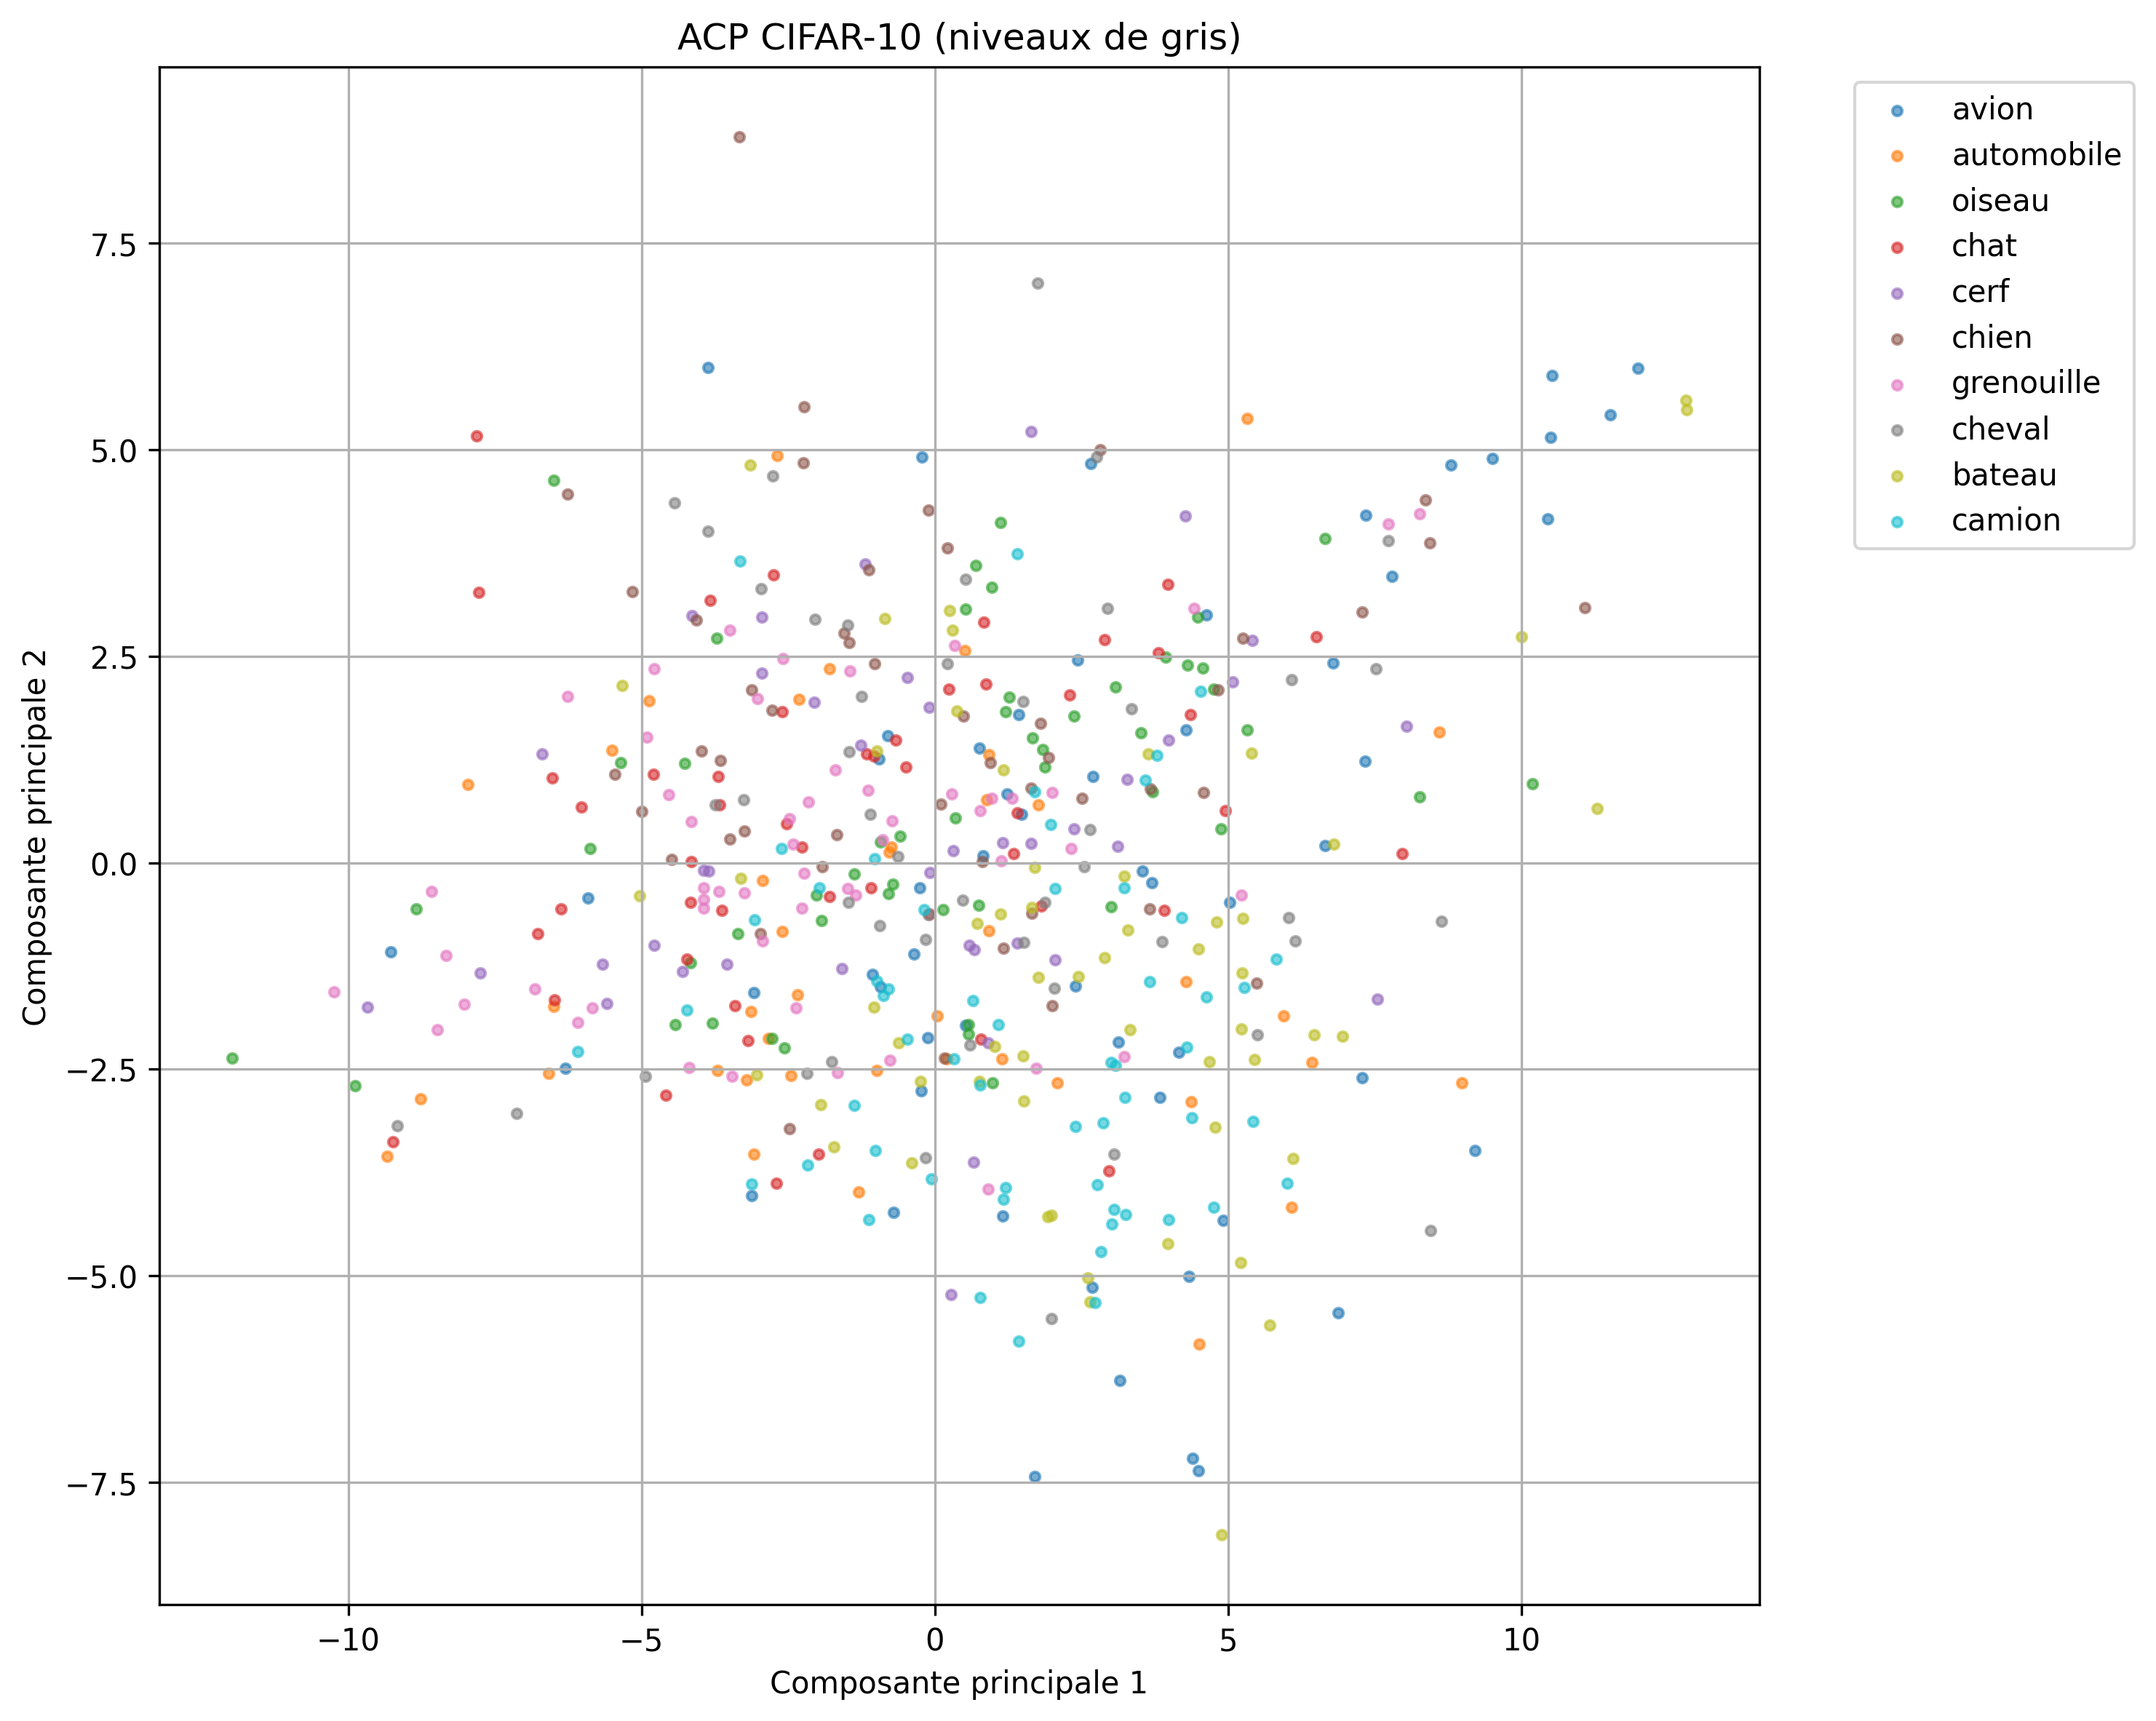
\includegraphics[width=0.6\textwidth]{cifar_acp.png}
    \caption{Représentation des données CIFAR-10 en 2 dimensions via ACP.}
    \label{fig:cifar_acp}
\end{figure}

% --- Figures CBIS-DDSM ---

\begin{figure}[H]
    \centering
    \begin{subfigure}[b]{0.48\textwidth}
        \includegraphics[width=\textwidth]{sorties/ddsm/mlp_confusion_05.png}
        \caption{MLP — seuil 0,5}
    \end{subfigure}
    \hfill
    \begin{subfigure}[b]{0.48\textwidth}
        \includegraphics[width=\textwidth]{sorties/ddsm/mlp_confusion_cal.png}
        \caption{MLP — seuil calibré ($\geq 80\,\%$ sensibilité)}
    \end{subfigure}
    \caption{Matrices de confusion du MLP sur CBIS-DDSM.}
    \label{fig:ddsm_mlp_cm}
\end{figure}

\begin{figure}[H]
    \centering
    \begin{subfigure}[b]{0.48\textwidth}
        \includegraphics[width=\textwidth]{sorties/ddsm/cnn_confusion_05.png}
        \caption{CNN from scratch — seuil 0,5}
    \end{subfigure}
    \hfill
    \begin{subfigure}[b]{0.48\textwidth}
        \includegraphics[width=\textwidth]{sorties/ddsm/cnn_confusion_cal.png}
        \caption{CNN from scratch — seuil calibré}
    \end{subfigure}
    \caption{Matrices de confusion du CNN from scratch sur CBIS-DDSM.}
    \label{fig:ddsm_cnn_cm}
\end{figure}

\begin{figure}[H]
    \centering
    \begin{subfigure}[b]{0.48\textwidth}
        \includegraphics[width=\textwidth]{sorties/ddsm/resnet_confusion_05.png}
        \caption{ResNet18 — seuil 0,5}
    \end{subfigure}
    \hfill
    \begin{subfigure}[b]{0.48\textwidth}
        \includegraphics[width=\textwidth]{sorties/ddsm/resnet_confusion_cal.png}
        \caption{ResNet18 — seuil calibré}
    \end{subfigure}
    \caption{Matrices de confusion du ResNet18 transfer learning sur CBIS-DDSM.}
    \label{fig:ddsm_resnet_cm}
\end{figure}

\begin{figure}[H]
    \centering
    \includegraphics[width=0.55\textwidth]{sorties/ddsm/mlp_convergence.png}
    \caption{Convergence du MLP sur CBIS-DDSM.}
    \label{fig:ddsm_mlp_conv}
\end{figure}

\begin{figure}[H]
    \centering
    \begin{subfigure}[b]{0.48\textwidth}
        \includegraphics[width=\textwidth]{sorties/ddsm/cnn_convergence.png}
        \caption{CNN from scratch}
    \end{subfigure}
    \hfill
    \begin{subfigure}[b]{0.48\textwidth}
        \includegraphics[width=\textwidth]{sorties/ddsm/resnet_convergence.png}
        \caption{ResNet18 transfer learning}
    \end{subfigure}
    \caption{Convergence (train / validation) des modèles CNN sur CBIS-DDSM.}
    \label{fig:ddsm_cnn_conv}
\end{figure}

\begin{figure}[H]
    \centering
    \begin{subfigure}[b]{0.48\textwidth}
        \includegraphics[width=\textwidth]{sorties/ddsm/ablation_train_convergence.png}
        \caption{Perte entraînement}
    \end{subfigure}
    \hfill
    \begin{subfigure}[b]{0.48\textwidth}
        \includegraphics[width=\textwidth]{sorties/ddsm/ablation_val_convergence.png}
        \caption{Perte validation}
    \end{subfigure}
    \caption{Étude d'ablation — Convergence des 5 configurations sur CBIS-DDSM ($128 \times 128$).
             Chaque courbe ajoute une technique de régularisation par rapport à la précédente.}
    \label{fig:ablation}
\end{figure}

\end{document}